\documentclass[tikz,border=5pt]{standalone}
\usepackage[UTF8]{ctex}
\usepackage{amsmath,amssymb}
\usetikzlibrary{arrows.meta,calc,decorations.pathreplacing,decorations.markings}
\tikzset{>=Stealth,line cap=round,line join=round,lab/.style={font=\small},traj/.style={blue!75!black,thick},aux/.style={gray!70,dashed,thin}}
\begin{document}
% 1: launch models; local angle measured from tangent, not radial.
\begin{tikzpicture}[scale=.83,font=\small]
\begin{scope}
\draw[thick](-.2,0)--(5.2,0);
\draw[->] (0,0)--(5.4,0) node[right]{$x$};
\draw[->] (0,0)--(0,3.4) node[above]{$y$};
\draw[traj,domain=0:4.5,samples=90] plot(\x,{1.08*\x-.24*\x*\x});
\draw[->,red!75!black,thick](0,0)--(1.35,1.46) node[above]{$v_0$};
\draw (.65,0) arc(0:47.2:.65);
\node at(.85,.30){$\theta$};
\fill(0,0)circle(1.6pt)node[below left]{$A$};
\draw[->,thick](4.65,2.6)--(4.65,1.8)node[midway,right]{$g$};
\node at(2.4,-.6){匀强重力};
\end{scope}
\begin{scope}[xshift=8cm,yshift=1.6cm]
\fill[gray!10](0,0)circle(1.45);
\draw[thick](0,0)circle(1.45);
\draw[aux](-1.45,0)arc(180:0:1.45 and .38);
\draw(-1.45,0)arc(180:360:1.45 and .38);
\fill(0,0)circle(1.5pt)node[below left]{$O$};
\fill(0,1.45)circle(1.5pt)node[left]{$A$};
\draw[thin](0,0)--(0,1.45)node[midway,left]{$R$};
\draw[aux](-.5,1.45)--(2.1,1.45);
\draw[->,red!75!black,thick](0,1.45)--({1.4*cos(38)},{1.45+1.4*sin(38)})node[above]{$v_0$};
\draw(.55,1.45)arc(0:38:.55);
\node at(.8,1.69){$\theta$};
\pgfmathsetmacro{\kk}{.9*cos(38)^2}
\pgfmathsetmacro{\cc}{.9*sin(38)*cos(38)}
\pgfmathsetmacro{\ret}{2*atan(\cc/(1-\kk))}
\draw[traj,domain=0:\ret,samples=100]plot({1.45*\kk*sin(\x)/(1+(\kk-1)*cos(\x)-\cc*sin(\x))},{1.45*\kk*cos(\x)/(1+(\kk-1)*cos(\x)-\cc*sin(\x))});
\pgfmathsetmacro{\qr}{1.45*\kk/(1+(\kk-1)*cos(50)-\cc*sin(50))}
\coordinate(Q)at({\qr*sin(50)},{\qr*cos(50)});
\draw[->,thick](Q)--($(Q)!.30!(0,0)$)node[pos=0,above right=6pt]{$gR^2/r^2$};
\node at(0,-2.2){球对称引力};
\end{scope}
\end{tikzpicture}
% 2: uniform field; d=2. Focus circle is not trajectory.
\begin{tikzpicture}[scale=1.35,font=\small]
\def\dd{2}
\def\ang{35}
\pgfmathsetmacro{\xv}{\dd*sin(2*\ang)}
\pgfmathsetmacro{\yv}{\dd*sin(\ang)^2}
\pgfmathsetmacro{\yf}{-\dd*cos(2*\ang)}
\pgfmathsetmacro{\xe}{4*\dd*sin(\ang)*cos(\ang)}
\draw[aux](0,0)circle(\dd);
\draw[thick](-2.2,\dd)--(4.45,\dd)node[right]{$y=d$};
\draw[->](-2.25,0)--(4.5,0)node[right]{$x$};
\draw[->](0,-2.2)--(0,2.45)node[above]{$y$};
\draw[traj,domain=0:\xe,samples=100]plot(\x,{tan(\ang)*\x-\x*\x/(4*\dd*cos(\ang)^2)});
\coordinate(A)at(0,0);\coordinate(V)at(\xv,\yv);\coordinate(F)at(\xv,\yf);
\pgfmathsetmacro{\xp}{3.10}
\pgfmathsetmacro{\yp}{tan(\ang)*\xp-\xp*\xp/(4*\dd*cos(\ang)^2)}
\coordinate(P)at(\xp,\yp);\coordinate(M)at(\xp,\dd);
\draw[thin,red!70!black](F)--(P)--(M);
\draw[thin] (A)--(F)node[midway,below]{$d$};
\draw[aux](V)--(F);
\node at({\xv-.52},.24){$p<0$};
\draw ($(M)+(-.12,0)$)--++(0,-.12)--++(.12,0);
\fill(A)circle(1.3pt)node[below left]{$A$};
\fill(V)circle(1.3pt)node[above left]{$V$};
\fill(F)circle(1.3pt)node[below right]{$F$};
\fill(P)circle(1.3pt)node[below right]{$P$};
\fill(M)circle(1.3pt)node[above]{$M$};
\node[gray!75]at(-1.40,-1.60){焦点圆};
\end{tikzpicture}
% 3: a physical above-ground ellipse arc and hidden mathematical continuation.
\begin{tikzpicture}[scale=2.35,font=\small]
\def\uu{.9}\def\ang{40}
\pgfmathsetmacro{\kk}{\uu*cos(\ang)^2}
\pgfmathsetmacro{\cc}{\uu*sin(\ang)*cos(\ang)}
\pgfmathsetmacro{\ret}{2*atan(\cc/(1-\kk))}
\pgfmathsetmacro{\dd}{\uu/(2-\uu)}
\pgfmathsetmacro{\fx}{\dd*sin(2*\ang)}
\pgfmathsetmacro{\fy}{1-\dd*cos(2*\ang)}
\def\pphi{35}
\pgfmathsetmacro{\rp}{\kk/(1+(\kk-1)*cos(\pphi)-\cc*sin(\pphi))}
\coordinate(O)at(0,0);\coordinate(A)at(0,1);
\coordinate(F)at(\fx,\fy);\coordinate(P)at({\rp*sin(\pphi)},{\rp*cos(\pphi)});
\fill[gray!12](O)circle(1);
\draw[aux,domain=\ret:360,samples=200]plot({\kk*sin(\x)/(1+(\kk-1)*cos(\x)-\cc*sin(\x))},{\kk*cos(\x)/(1+(\kk-1)*cos(\x)-\cc*sin(\x))});
\draw[thick](O)circle(1);
\draw[aux](-1,0)arc(180:0:1 and .20);
\draw[thin](-1,0)arc(180:360:1 and .20);
\draw[traj,domain=0:\ret,samples=150]plot({\kk*sin(\x)/(1+(\kk-1)*cos(\x)-\cc*sin(\x))},{\kk*cos(\x)/(1+(\kk-1)*cos(\x)-\cc*sin(\x))});
\draw[thin](O)--(A)node[midway,left]{$R$};
\draw[thin,red!70!black](A)--(F)node[midway,above]{$D$};
\draw[thin,red!70!black](O)--(P)node[pos=.40,left]{$r$};
\draw[thin,red!70!black](F)--(P)node[midway,right]{$FP$};
\draw[aux](-.3,1)--(.75,1);
\draw[->](A)--++(.48,.4)node[above left]{$v_0$};
\foreach \N in{O,A,F,P}\fill(\N)circle(.65pt);
\node[below left]at(O){$O$};
\node[above left]at(A){$A$};
\node[below right]at(F){$F$};
\node[above right]at(P){$P$};
\coordinate(B)at({sin(\ret)},{cos(\ret)});
\fill(B)circle(.65pt)node[below right]{$B$};
\node at(-1.0,-1.25){首次落点 $B$};
\end{tikzpicture}
% 4: envelope geometry. A,F,P ordered along a straight segment, not the trajectory.
\begin{tikzpicture}[scale=1.72,font=\small]
\def\ss{4}\def\dd{1.5}\def\phi{65}
\pgfmathsetmacro{\rr}{(\ss*\ss-1)/(2*(\ss-cos(\phi)))}
\pgfmathsetmacro{\px}{\rr*sin(\phi)}
\pgfmathsetmacro{\py}{\rr*cos(\phi)}
\pgfmathsetmacro{\dist}{\ss-\rr}
\pgfmathsetmacro{\fx}{\dd*\px/\dist}
\pgfmathsetmacro{\fy}{1+\dd*(\py-1)/\dist}
\coordinate(O)at(0,0);\coordinate(A)at(0,1);
\coordinate(F)at(\fx,\fy);\coordinate(P)at(\px,\py);
\fill[gray!10](O)circle(1);
\draw[thick](O)circle(1);
\draw[blue!75!black,thick](0,.5)ellipse({sqrt(3.75)} and 2);
\draw[aux](A)circle(\dd);
\draw[thin,red!75!black](O)--(P)node[pos=.30,above left]{$r$};
\draw[thin,red!75!black](A)--(F)--(P);
\node[above]at($(A)!.48!(F)$){$D$};
\node[above right=11pt]at($(F)!.5!(P)$){$FP$};
\draw[decorate,decoration={brace,mirror,amplitude=4pt}]($(A)+(0,-.13)$)--($(P)+(0,-.13)$)node[midway,below=5pt]{$s$};
\foreach \N in{O,A,F,P}\fill(\N)circle(.75pt);
\node[below left]at(O){$O$};
\node[above left]at(A){$A$};
\node[above left=3pt]at(F){$F$};
\node[below right]at(P){$P$};
\pgfmathsetmacro{\nx}{\px/\rr+\px/\dist}
\pgfmathsetmacro{\ny}{\py/\rr+(\py-1)/\dist}
\pgfmathsetmacro{\nn}{sqrt(\nx*\nx+\ny*\ny)}
\draw[->,thin](P)--++({.75*\nx/\nn},{.75*\ny/\nn})node[right]{共同法向};
\node at(-1.10,-1.8){$r+s=S$};
\end{tikzpicture}
% 5: projected surfaces of revolution. x=x_world, y=z_world+.30*y_world.
% Their projected silhouettes and rings use the same oblique projection.
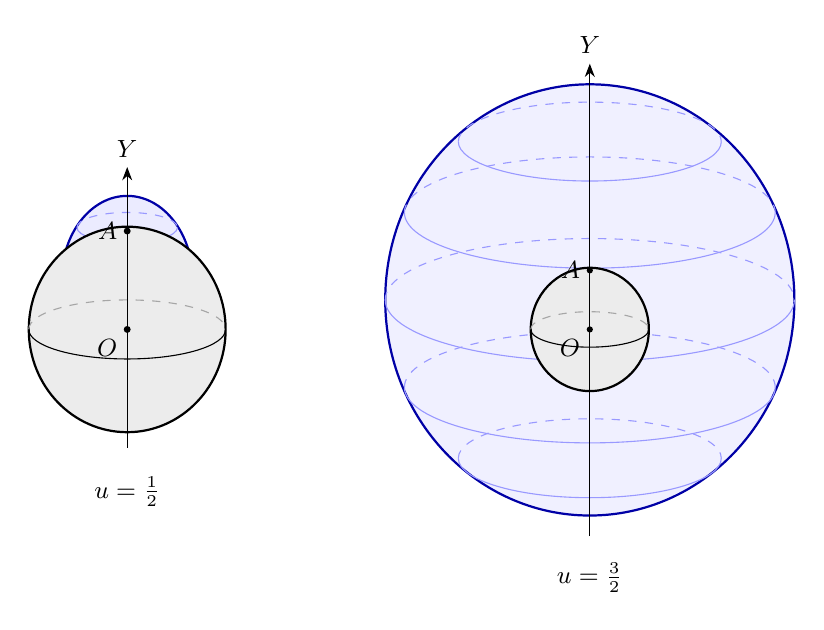
\begin{tikzpicture}[font=\small,scale=1.25]
\begin{scope}[xshift=0cm]
\def\aa{.833333}\def\bb{.666667}
\pgfmathsetmacro{\ay}{sqrt(\aa*\aa+.09*\bb*\bb)}
\fill[blue!8](0,.5)ellipse({\bb} and {\ay});
\draw[blue!65!black,thick](0,.5)ellipse({\bb} and {\ay});
\foreach \lat in{-40,0,40}{
\pgfmathsetmacro{\rad}{\bb*cos(\lat)}
\pgfmathsetmacro{\yy}{.5+\aa*sin(\lat)}
\draw[blue!40,dashed](-\rad,\yy)arc(180:0:{\rad} and {.3*\rad});
\draw[blue!40](-\rad,\yy)arc(180:360:{\rad} and {.3*\rad});
}
\fill[gray!15](0,0)ellipse(1 and {sqrt(1.09)});
\draw[thick](0,0)ellipse(1 and {sqrt(1.09)});
\draw[aux](-1,0)arc(180:0:1 and .3);
\draw[thin](-1,0)arc(180:360:1 and .3);
\draw[->,thin](0,-1.2)--(0,1.65)node[above]{$Y$};
\fill(0,0)circle(1pt)node[below left]{$O$};
\fill(0,1)circle(1pt)node[left]{$A$};
\node at(0,-1.65){$u=\frac12$};
\end{scope}
\begin{scope}[xshift=4.7cm,scale=.60]
\def\aa{3.5}\def\bb{3.464102}
\pgfmathsetmacro{\ay}{sqrt(\aa*\aa+.09*\bb*\bb)}
\fill[blue!6](0,.5)ellipse({\bb} and {\ay});
\draw[blue!65!black,thick](0,.5)ellipse({\bb} and {\ay});
\foreach \lat in{-50,-25,0,25,50}{
\pgfmathsetmacro{\rad}{\bb*cos(\lat)}
\pgfmathsetmacro{\yy}{.5+\aa*sin(\lat)}
\draw[blue!40,dashed](-\rad,\yy)arc(180:0:{\rad} and {.3*\rad});
\draw[blue!40](-\rad,\yy)arc(180:360:{\rad} and {.3*\rad});
}
\fill[gray!15](0,0)ellipse(1 and {sqrt(1.09)});
\draw[thick](0,0)ellipse(1 and {sqrt(1.09)});
\draw[aux](-1,0)arc(180:0:1 and .3);
\draw[thin](-1,0)arc(180:360:1 and .3);
\draw[->,thin](0,-3.5)--(0,4.5)node[above]{$Y$};
\fill(0,0)circle(1.5pt)node[below left]{$O$};
\fill(0,1)circle(1.5pt)node[left]{$A$};
\node at(0,-4.2){$u=\frac32$};
\end{scope}
\end{tikzpicture}
% 6: critical escape (u=2), meridian section. Reachable side is above boundary.
\begin{tikzpicture}[scale=1.15,font=\small]
\fill[blue!7](-3.3,{-1.7225})--plot[domain=-3.3:3.3,samples=140](\x,{1-\x*\x/4})--(3.3,3.1)--(-3.3,3.1)--cycle;
\fill[gray!16](0,0)circle(1);
\draw[thick](0,0)circle(1);
\draw[traj,domain=-3.3:3.3,samples=140]plot(\x,{1-\x*\x/4});
\draw[->,red!70!black,thick](0,1)--(1.2,1)node[above]{$v_0$};
\draw[->](0,-1.25)--(0,3.3)node[above]{$OA$};
\coordinate(O)at(0,0);\coordinate(A)at(0,1);
\coordinate(P)at(2,0);
\draw[thin](O)--(P)node[pos=.70,below]{$r_t$};
\draw[thin](0,.42)arc(90:0:.42);
\node at(.42,.38){$\varphi$};
\fill(O)circle(1.3pt)node[below left]{$O$};
\fill(A)circle(1.3pt)node[above left]{$A$};
\fill(P)circle(1.3pt)node[below right]{$P$};
\draw[blue!45!black,domain=0:78,samples=80,postaction={decorate},decoration={markings,mark=at position .65 with {\arrow{Stealth}}}]plot({2*cos(20)^2*sin(\x)/(1+cos(40+\x))},{2*cos(20)^2*cos(\x)/(1+cos(40+\x))});
\node at(-2.0,2.5){外行可达侧};
\node at(2.4,-1.65){$u=2$};
\end{tikzpicture}
\end{document}
